\chapter{OPIS TECHNICZNY}
\label{chapter:opis_techniczny}


\section{Aplikacja wit.ai}
W ramach projektu została stworzona aplikacja w systemie \textit{wit.ai}. Wit.ai to platforma do tworzenia interfejsów interaktywnych, która pozwala na budowanie aplikacji, które rozumieją naturalny język. Wit.ai pozwala na tworzenie modeli językowych, które są w stanie rozpoznawać intencje użytkownika na podstawie zdefiniowanych przez programistę fraz. Aplikacja ta jest wykorzystywana w projekcie do rozpoznawania intencji użytkownika na podstawie zdefiniowanych przez programistę fraz.

\subsection{Intencje i encje}

W celu nauczenia modelu językowego aplikacji wit.ai, należy zdefiniować intencje (ang. \textit{intents}), które mają być rozpoznawane przez aplikację. Intencje to frazy, które użytkownik może napisać, a które mają być zrozumiane przez aplikację. Każda intencja może zawierać wiele przykładów fraz, które są z nią związane. Przykładowe intencje, które zostały zdefiniowane w aplikacji wit.ai to:
\begin{itemize}
    \item \textit{add\_product\_to\_cart} - intencja dodania produktu do koszyka,
    \item \textit{remove\_product\_from\_cart} - intencja usunięcia produktu z koszyka,
    \item \textit{check\_cart} - intencja sprawdzenia zawartości koszyka,
    \item \textit{check\_item\_prices} - intencja sprawdzenia cen produktów,
    \item \textit{check\_item\_price\_in\_store} - intencja sprawdzenia ceny produktu w sklepie
\end{itemize}

Poza intencjami, w aplikacji wit.ai definiuje się również encje (ang. \textit{entities}). Encje to frazy, które mają być rozpoznawane przez aplikację jako konkretne wartości. Encje pomagają również w wykryciu intencji użytkownika. Przykładowe encje, które zostały zdefiniowane w aplikacji wit.ai to:
\begin{itemize}
    \item \textit{product} - encja reprezentująca nazwę produktu,
    \item \textit{store} - encja reprezentująca nazwę sklepu,
    \item \textit{view} - encja reprezentująca widok w aplikacji,
    \item \textit{category} - encja reprezentująca nazwę kategorii produktów
\end{itemize}

Po zdefiniowaniu intencji i encji, aplikacja wit.ai pozwala na trenowanie modelu językowego. Trenowanie modelu polega na przesłaniu do aplikacji wit.ai przykładów fraz, które mają być rozpoznawane przez aplikację. Po przesłaniu przykładów, aplikacja wit.ai trenuje model językowy. Po wstępnym treningu, aplikacja stara się sama sugerować intencje w procesie trenowania modelu. Pozwala to na sprawdzanie w czasie rzeczywistym, czy model językowy poprawnie rozpoznaje encje i intencje. Przykładowe frazy wykorzystane w procesie trenowania modelu to:
\begin{itemize}
    \item \textit{Where to buy apples}
    \item \textit{Remove cheese from cart},
    \item \textit{My app is stuck on loading},
    \item \textit{Is there dairy in castorama?}
\end{itemize}

\subsection{Kreator}

Wytrenowany model należy zaprogramować. W tym celu wit.ai udostępnia kreator (ang. \textit{composer}), który pozwala na zdefiniowanie akcji, które mają być wykonywane po rozpoznaniu intencji przez aplikację. Przykładowe akcje, które zostały zdefiniowane w aplikacji wit.ai przedstawiono na rysunku \ref{fig:wit_ai_composer}.

\begin{figure}[H]
    \centering
    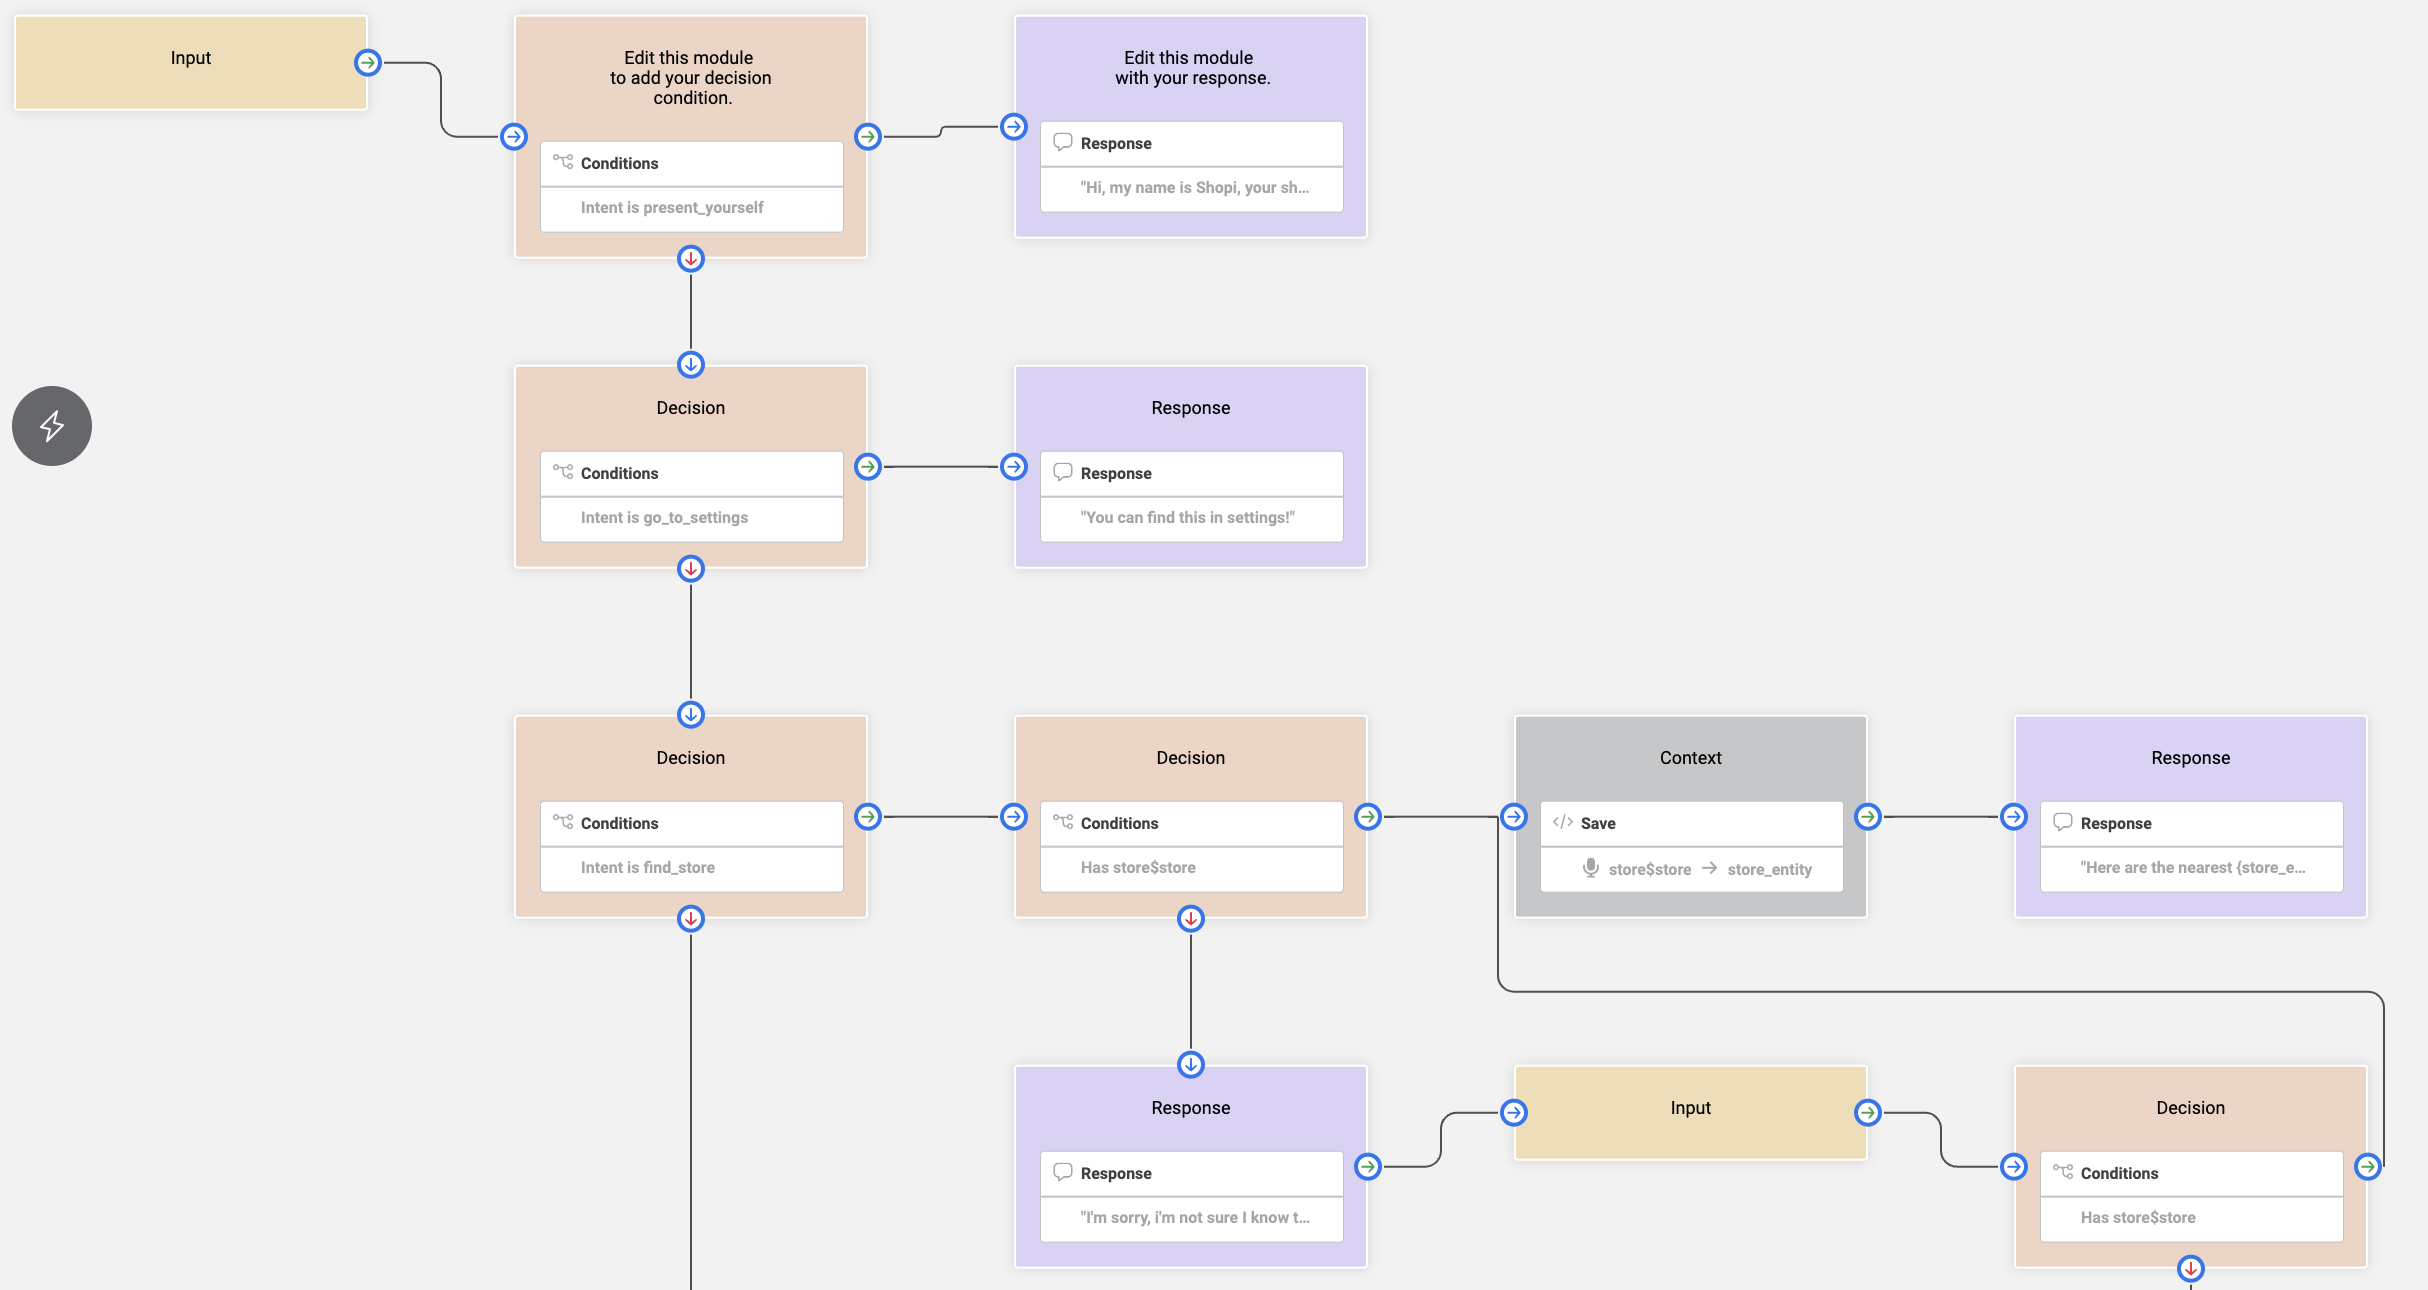
\includegraphics[width=0.8\textwidth]{images/witai_composer.png}
    \caption{Kreator aplikacji wit.ai}
    \label{fig:wit_ai_composer}
\end{figure}

\subsubsection{Akcje}

W ramach kreatora dostępne są 4 moduły blokowe definiujące akcje. Są to:
\begin{itemize}
    \item \textit{Decision} - moduł decydujący o dalszym przebiegu akcji,
    \item \textit{Context} - moduł przechowujący kontekst akcji,
    \item \textit{Input} - moduł pobierający dane wejściowe,
    \item \textit{Response} - moduł generujący odpowiedź.
\end{itemize}

\subsubsection{Decision}

Moduł \textit{Decision} pozwala na zdefiniowanie warunków, które muszą być spełnione, aby akcja mogła zostać wykonana. Dostępne są poniższe warunki:
\begin{itemize}
    \item \textit{Intent} - sprawdza, czy intencja użytkownika jest zgodna z zdefiniowaną intencją,
    \item \textit{Entity} - sprawdza, czy encja użytkownika jest zgodna z zdefiniowaną encją,
    \item \textit{Context} - sprawdza, czy kontekst akcji jest zgodny z zdefiniowanym kontekstem,
    \item \textit{Trait} - sprawdza, czy cecha akcji jest zgodna z zdefiniowaną cechą.
    \item \textit{Not/And/Or} - służy do łączenia warunków.
\end{itemize}

\subsubsection{Context}
Moduł \textit{Context} pozwala na zdefiniowanie kontekstu akcji. Kontekst to zmienna, która przechowuje informacje o stanie akcji. Kontekst może być wykorzystywany w kolejnych akcjach. W ramach tego modułu możn a wykonać 4 akcje:
\begin{itemize}
    \item \textit{Set} - ustawia wartość kontekstu,
    \item \textit{Save} - zapisuje rozpoznaną encję do kontekstu,
    \item \textit{Copy} - kopiuje wskazaną wartość kontekstu,
    \item \textit{Clear} - czyści kontekst.
\end{itemize}

\subsubsection{Input}
Moduł \textit{Input} pozwala na pobranie danych wejściowych. Jest on wykorzystywany na początku kreatora, w celu przyjęcia wiadomości od użytkownika. Można go również użyć do uzyskania dodatkowych informacji od użytkownika.

\subsubsection{Response}
Moduł \textit{Response} pozwala na zdefiniowanie odpowiedzi, która ma zostać zwrócona do użytkownika. W odpowiedzi można wykorzystać zmienne zdefiniowane w kontekście akcji. Można zwrócić tekst, obraz, dźwięk, link, czy dowolny inny format. Oprócz tego, można również zwrócić nazwę funkcji, która ma zostać wykonana po zakończeniu akcji.


\subsection{Testowanie i publikacja}
Po zdefiniowaniu akcji, aplikacja wit.ai pozwala na przetestowanie modelu językowego. W tym celu można wpisać dowolną frazę, a aplikacja zwróci intencję oraz encje, które rozpoznała. Po zakończeniu testowania, model językowy można opublikować. Po opublikowaniu modelu, aplikacja wit.ai generuje token, który pozwala na integrację modelu z dowolną aplikacją. Token ten jest wykorzystywany w aplikacji mobilnej, aby komunikować się z modelem językowym.


\section{Serwer}
Serwer jest odpowiedzialny za przetwarzanie żądań użytkownika, a także za komunikację z bazą danych. Serwer został zaimplementowany w języku JavaScript, z wykorzystaniem struktury (ang. \textit{framework}) Express.js. Express.js to minimalistyczny framework, który pozwala na tworzenie aplikacji internetowych w języku JavaScript. Serwer nasłuchuje na zapytania HTTP, a następnie przetwarza je i zwraca odpowiedź. Serwer komunikuje się z bazą danych PostgreSQL. 

\subsection{Struktura serwera}
